\chapter{Results}
\label{chap:results}

In this chapter we present results from the evaluation phase.

\section{Data separation}
Not written yet.

\section{Query support}
The set of important queries defined in table~\ref{tab:queries} has been implemented for both archive prototypes. Results from the first iteration are presented in table~\ref{tab:archivequeries}. These are just the initial presentation of the results.
\begin{table}[h]
\begin{tabular}{|l|l|l|}
\hline
\textbf{High level query}                & \textbf{Supported} & \textbf{Comment}           \\ \hline
Get build                                    & Y                                                                                        &                            \\ \hline
Get build information                        & Y                                                                                        &                            \\ \hline
Get build for root test suite                & Y                                                                                        &                            \\ \hline
Get trouble reports for build                & Y                                                                                        &                            \\ \hline
Get trouble report fixes for build           & Y                                                                                        &                            \\ \hline
Get trouble reports for product and revision & Y                                                                                        &                            \\ \hline
Get test suite children                      & Y                                                                                        &                            \\ \hline
Get test case in build                       & Y                                                                                        &                            \\ \hline
Get test suite in build                      & Y                                                                                        &                            \\ \hline
Get root test suite for test case/test suite & Y                                                                                        &                            \\ \hline
Get test case by name                        & Y                                                                                        & Used for test case history \\ \hline
Get test suite for test case                 & Y                                                                                        &                            \\ \hline
Get test case history                        & P                                                                                        & Tags not supported         \\ \hline
Get test tree                                & P                                                                                        & Runs slow for large trees  \\ \hline
\end{tabular}
\caption{Possible values in the supported column are yes/no/partially.}
\label{tab:archivequeries}
\end{table}

\section{Schema evolution}
Not yet addressed

\section{Scalability}
\subsection{Disk usage}
Disk usage after migration of live databases of different sizes are presented in figure~\ref{fig:disc}. Currently, migrations with data sets of around 100 million and 400 million job events have been performed. 
\begin{figure}[h!]
\centering
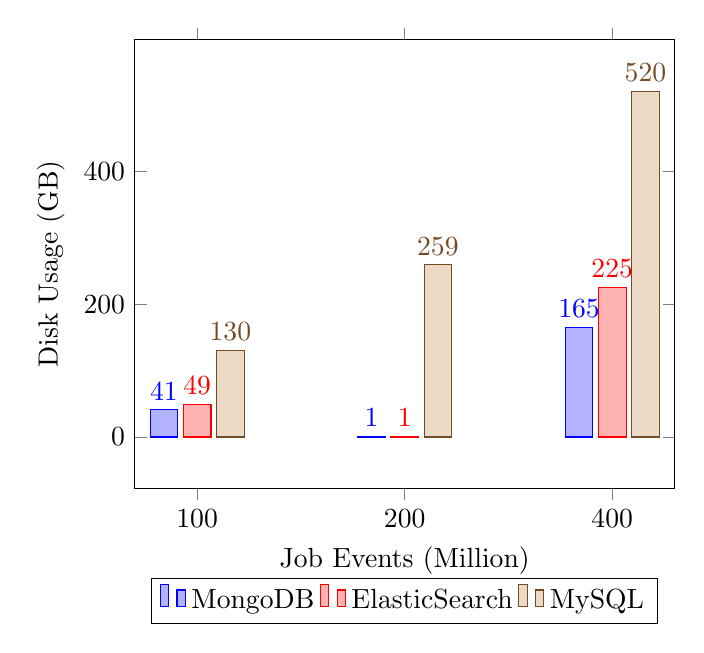
\begin{tikzpicture}
\begin{axis}[
    ybar,
    enlargelimits=0.15,
    legend style={at={(0.5,-0.2)},
      anchor=north,legend columns=-1, },
    xlabel={Job Events (Million)},
    ylabel={Disk Usage (GB)},
    symbolic x coords={100,200,400},
    xtick=data,
    nodes near coords,
    nodes near coords align={vertical},
    ]
\addplot coordinates {(100,41) (200,1) (400,165)};
\addplot coordinates {(100,49) (200,1) (400,225)};
\addplot coordinates {(100,130) (200,259) (400,520)};
\legend{MongoDB,ElasticSearch,MySQL}
\end{axis}
\end{tikzpicture}
\caption{Disk usage}
\label{fig:disc}
\end{figure}
\subsection{Memory utilization}
Working set estimations are presented in figure~\ref{fig:ws}. We have done initial estimations of the working set for MongoDB with manual testing. As long as custom indexes defined on the job event collection fit in RAM, the database is stable and can respond to queries where indexes can be utilized. The working set estimation is the summed size of the custom indexes.
\begin{figure}[h!]
\centering
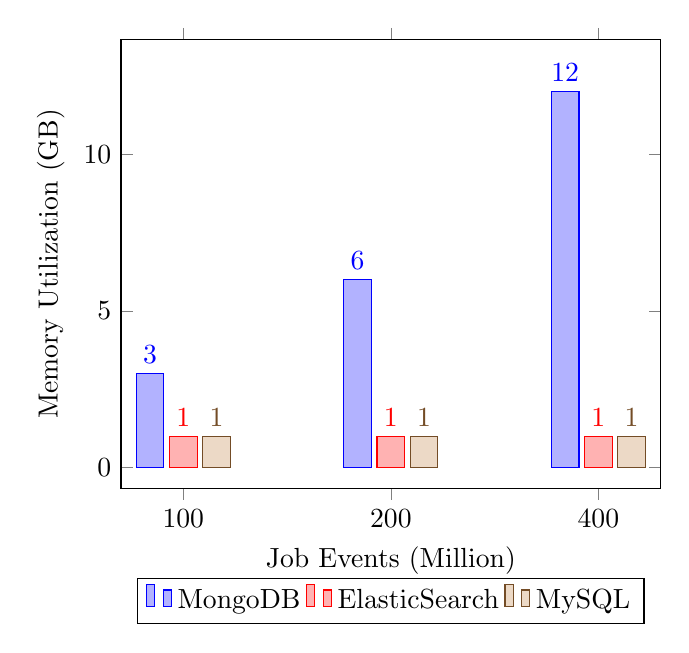
\begin{tikzpicture}
\begin{axis}[
    ybar,
    enlargelimits=0.15,
    legend style={at={(0.5,-0.2)},
      anchor=north,legend columns=-1, },
    xlabel={Job Events (Million)},
    ylabel={Memory Utilization (GB)},
    symbolic x coords={100,200,400},
    xtick=data,
    nodes near coords,
    nodes near coords align={vertical},
    ]
\addplot coordinates {(100,3) (200,6) (400,12)};
\addplot coordinates {(100,1) (200,1) (400,1)};
\addplot coordinates {(100,1) (200,1) (400,1)};
\legend{MongoDB,ElasticSearch,MySQL}
\end{axis}
\end{tikzpicture}
\caption{Working set estimation}
\label{fig:ws}
\end{figure}
\subsection{Insertion time}
Not yet addressed
\subsection{Horizontal Scalability}
Not yet addressed
Här borde vi kunna skriva tekniska saker, men från de tekniska saker dra slutsater i Discussion som svarar på om dessa tekniker ger något business value?
\subsubsection{ElasticSearch}






